\section{JavaScript Semantics Specialization with Syntactic Views}\label{sec:formal}

In this section, we introduce a JavaScript semantics specialization with
syntactic views.  We first introduce $\ires$ as a specification language to
describe JavaScript semantics. To provide options to select target semantics, we
also introduce syntactic views as an abstraction of JavaScript ASTs.  Then, we
define a JavaScript semantics specialization with syntactic views as a partial
evaluation of $\ires$ programs, which is a combination of static analysis and
program transformation. Finally, we prove the semantics preservation of the
partial evaluation.

\subsection{$\ires$: Intermediate Representations for ECMAScript}

We first introduce $\ires$, an \textbf{I}ntermediate \textbf{R}epresentations
for \textbf{E}CMA\textbf{S}cript, as a specification language for JavaScript to
describe JavaScript semantics. We define its abstract syntax, states, and
concrete semantics in the remainder of this section.

\subsubsection{Abstract Syntax}

\[
  \begin{array}{lr@{~}c@{~}c@{~}c@{~}l}
    \text{Programs} & \progset &\ni& \prog &=& (\istset, \getfunc, \getinst,
    \getnext)\\

    \text{Functions} & \funcset &\ni& \func &::=&
    \kwdef \; \kwrl \varx^* \kwrr \; \lab\\

    \text{Variables} & \varset &\ni& \varx\\

    \text{Instructions} & \instset &\ni& \inst &::=&
    \refer \kweq \expr \mid
    \varx \kweq \kwcl \kwcr \mid
    \varx \kweq \expr \kwrl \expr^* \kwrr \mid \\&&&&&
    \kwif \; \expr \; \lab \; \lab \mid
    \kwret \; \expr\\

    \text{Labels} & \labset &\ni& \lab\\

    \text{Expressions} & \exprset &\ni& \expr &::=&
    \pval \mid
    \op \kwrl \expr^* \kwrr \mid
    \refer\\

    \text{References} & \referset &\ni& \refer &::=&
    \varx \mid \expr \kwsl \expr \kwsr\\
  \end{array}
\]

An $\ires$ program $\prog = (\istset, \getfunc, \getinst, \getnext) \in \progset $
consists of initial states and three mappings; $\getfunc: \labset \rightarrow
\funcset$ and $\getinst: \labset \rightarrow \instset$ map labels to their
functions and instructions, respectively, and $\getnext: \labset \rightarrow
\labset$ maps labels to their next labels, where a label $\lab \in \labset$
denotes a program point.  A function $\func \in \funcset$ is defined with its
parameters and body label.  For presentation brevity, we assume that no global
or captured variables exist in this paper.  An instruction $\inst \in \instset$
is an assignment $\refer \kweq \expr$, an object allocation $\varx \kweq \kwcl \kwcr$, a
function call $\varx \kweq \expr \kwrl \expr^* \kwrr$, a branch $\kwif \; \expr \;
\lab \; \lab$, or a return instruction $\kwret \; \expr$.  An invocation of an
abstract algorithm in ECMAScript is compiled to a function call instruction with
a new temporary variable.  We represent loops using branch instructions with
cyclic pointing of labels in $\getnext$.  An expression is a primitive value
$\pval$, an operation $\op \kwrl \expr^* \kwrr$, or a reference $\refer$.  A
reference is a variable $\varx$ or an object field $\expr \kwsl \expr \kwsr$.
We write $\expr.\varf$ to briefly represent $\expr \kwsl \code{"f"} \kwsr$.


\subsubsection{States}

\[
  \begin{array}{lr@{~}c@{~}l@{~}c@{~}l}
    \text{States} & \st &\in& \stset &=&
    \labset \times \ctxtset^* \times \heapset \times \envset\\

    \text{Calling Contexts} & \ctxt &\in& \ctxtset &=&
    \labset \times \envset \times \varset\\

    \text{Heaps} & \heap &\in& \heapset &=&
    \addrset \finmap \objset\\

    \text{Objects} & \obj &\in& \objset &=&
    \strset \finmap \valset\\

    \text{Environments} & \env &\in& \envset &=&
    \varset \finmap \valset\\

    \text{Values} & \val &\in& \valset &=&
    \pvalset \uplus \addrset \uplus \treeset \uplus \funcset\\

    \text{Primitive Values} & \pval &\in& \pvalset &=&
    \boolset \uplus \intset \uplus \strset \uplus \cdots\\

    \text{JavaScript ASTs} & \tree &\in& \treeset\\
  \end{array}
\]

States $\stset$ consist of labels $\labset$, calling context stacks
$\ctxtset^*$, heaps $\heapset$, and environments $\envset$.  A calling context
$\ctxt \in \ctxtset$ consists of a label denoting the return point, a caller's
environment, and a return variable.  A heap $\heap \in \heapset$ is a finite
mapping from addresses to objects, and an object $\obj \in \objset$ is a finite
mappings from strings to values.  Each object allocation $\kwcl \kwcr$ creates a
unique address $\addr \in \addrset$ different from existing addresses.  An
environment $\env \in \envset$ is a finite mapping from variables to values. A
value $\val \in \valset$ is a primitive value $\pval \in \pvalset$ (e.g., a
boolean value $\bool \in \boolset$, an integer $k \in \intset$, or a string
$\str \in \strset$), an address $\addr \in \addrset$, a JavaScript AST $\tree
\in \treeset$, or a function $f \in \funcset$.

$\ires$ is a specification language for JavaScript that treats JavaScript ASTs
as its values. To handle JavaScript ASTs in $\ires$, we define them with tree
nodes $\nodeset$ as follows:
\[
  \begin{array}{l@{~}c@{~}l@{~}c@{~}l}
    \treeset &\ni& \tree &::=& \ty_k \langle \node^* \rangle\\
    \nodeset &\ni& \node &::=& \str \mid \tree\\
  \end{array}
\]
A JavaScript AST $\ty_k \langle \node_1, \cdots, \node_n \rangle$ denotes $k$-th
alternative in the syntactic production of nonterminal symbol $\ty$ with
multiple tree nodes $\node_1, \cdots, \node_n$.  A tree node is a string for a
terminal symbol or another tree for a nonterminal symbol. We define several
notations to easily deal with JavaScript ASTs.  The notation $\ty_k.\eval$ denotes
an \esalg{Evaluation} function of $k$-th alternative in the production $\ty$.
Similarly, the notation $\tree.\eval$ denotes the \esalg{Evaluation} function of
the AST $\tree$, and it is same with $\ty_k.\eval$ when $\tree = \ty_k \langle
\cdots \rangle$. The \esalg{Evaluation} of each AST takes the AST itself and its
tree nodes that are nonterminals as arguments.  The notation $\getsubs(\tree)$
denotes tree nodes that are subtrees of $\tree$.  For example,
Figure~\ref{fig:coalesce-prod} shows a syntactic production for coalesce
expressions.  Consider the following JavaScript coalesce expression:
\begin{lstlisting}[style=JS]
                    42 ?? true
\end{lstlisting}
Then, the following AST is produced as its parsing result:
\[
  \begin{array}{lcl}
    \tree_0 &=&
    \essyn{CoalesceExpression}_0 \langle \tree_1, \code{"??"}, \tree_2 \rangle\\

    \tree_1 &=&
    \essyn{CoalesceExpressionHead}_1 \langle \tree_3 \rangle\\

    \tree_2 &=&
    \essyn{BitwiseORExpression}_0 \langle \cdots \rangle\\

    \tree_3 &=&
    \essyn{BitwiseORExpression}_0 \langle \cdots \rangle\\
  \end{array}
\]
\begin{figure}[H]
  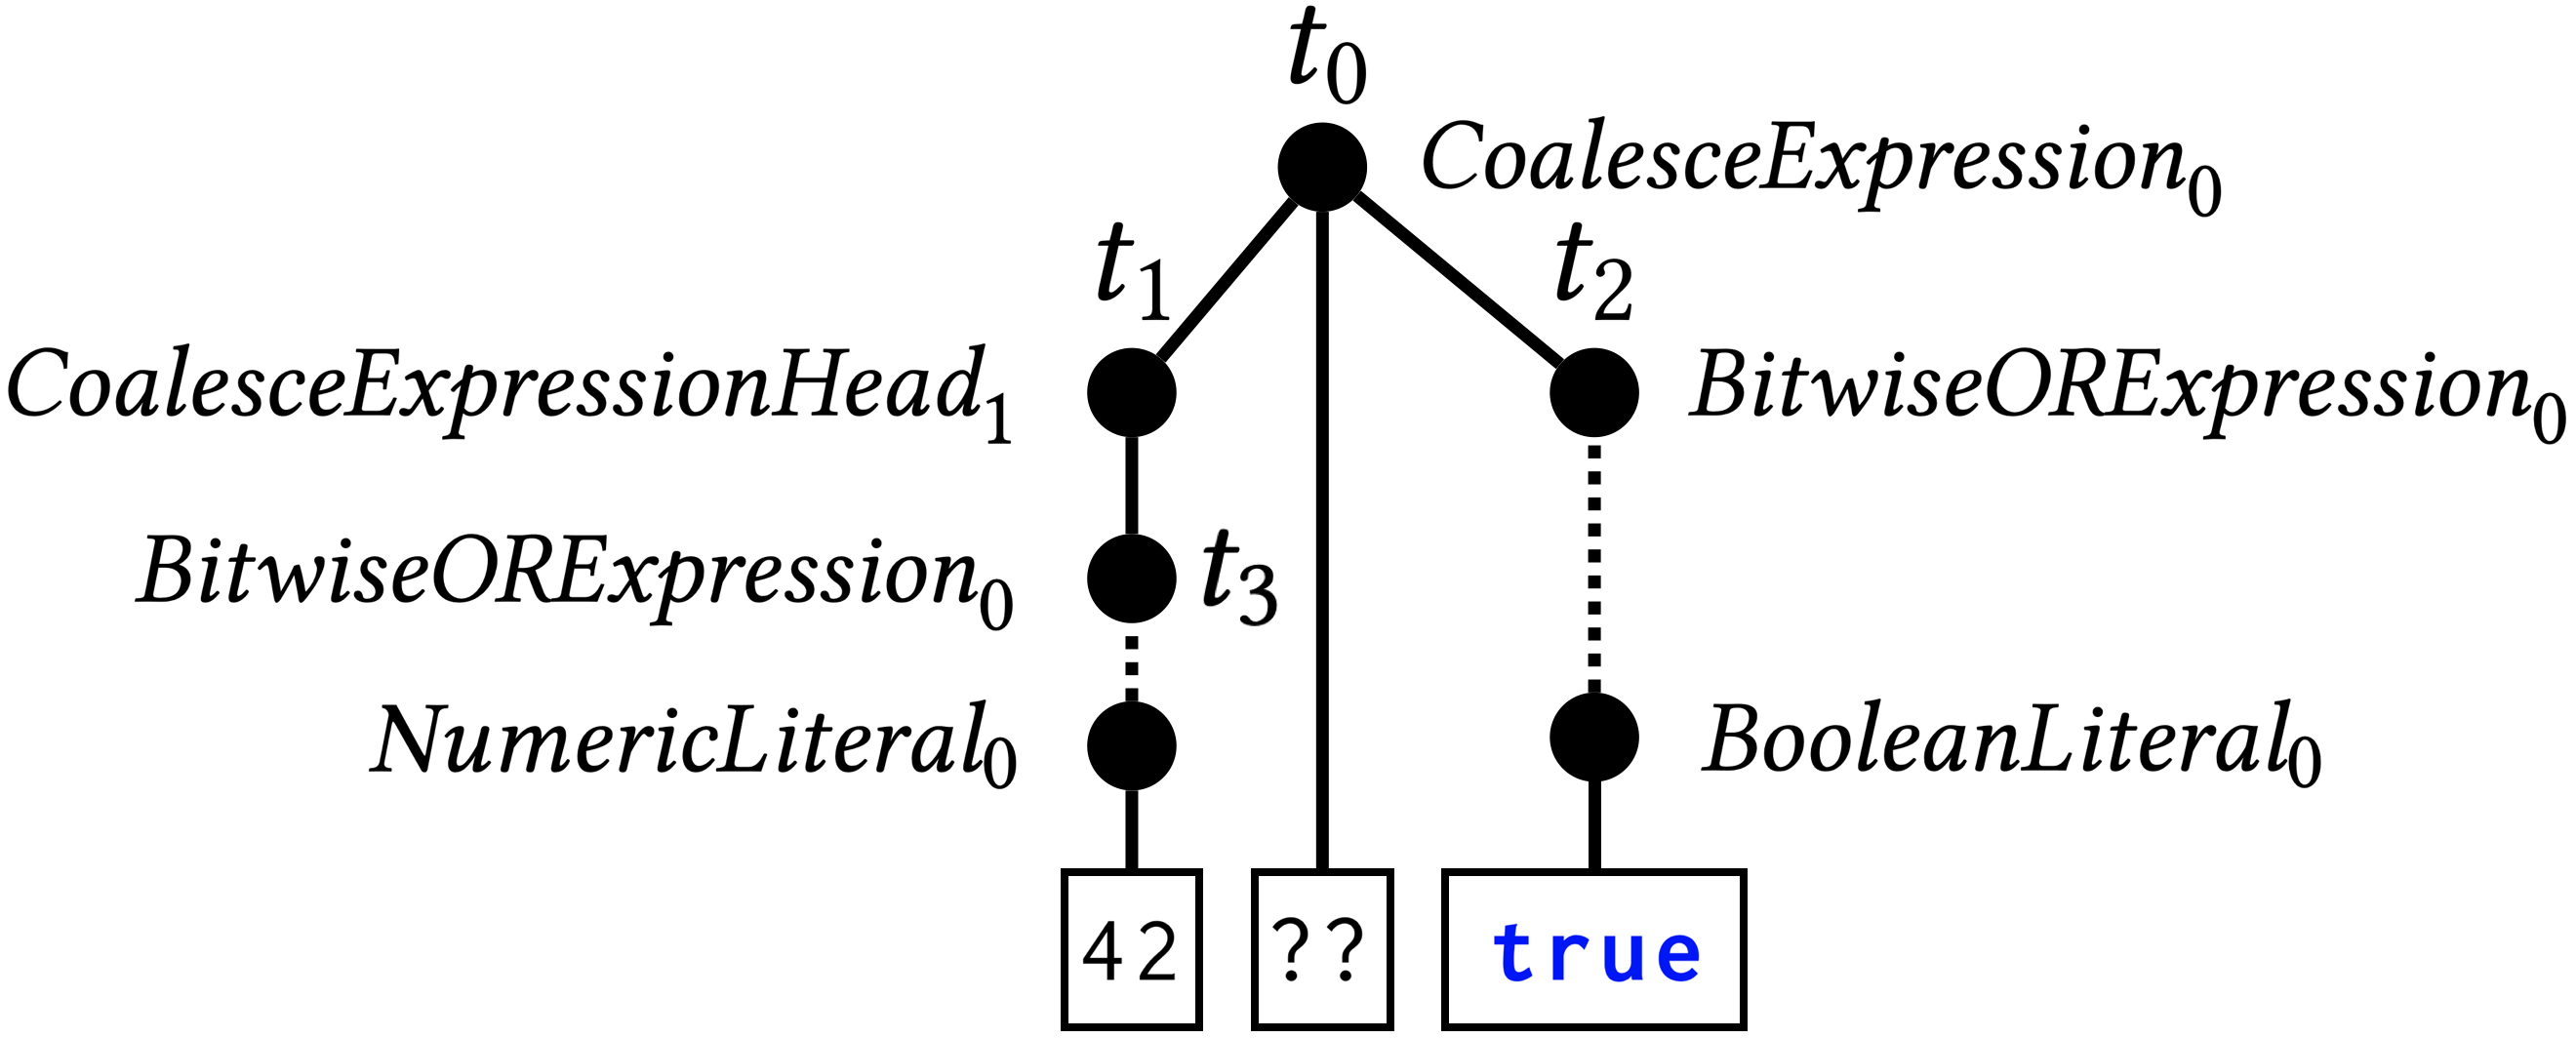
\includegraphics[width=.8\columnwidth]{img/ast-example.png}
\end{figure}
\noindent Its \esalg{Evaluation} function $\essyn{CoalesceExpression}_0.\eval$
takes three subtrees as arguments annotated by $\tree_0$, $\tree_1$, and
$\tree_2$ in the figure. The ASTs $\tree_0$, $\tree_1$, $\tree_2$, and $\tree_3$
are subtrees of $\tree_0$ (i.e., $\tree_0 \subtree \tree_0, \cdots, \tree_3
\subtree \tree_0$), and $\getsubs(\tree_0) = [\tree_1, \tree_2] \wedge
\getsubs(\tree_1) = [\tree_3]$.


\begin{figure}
  \centering
  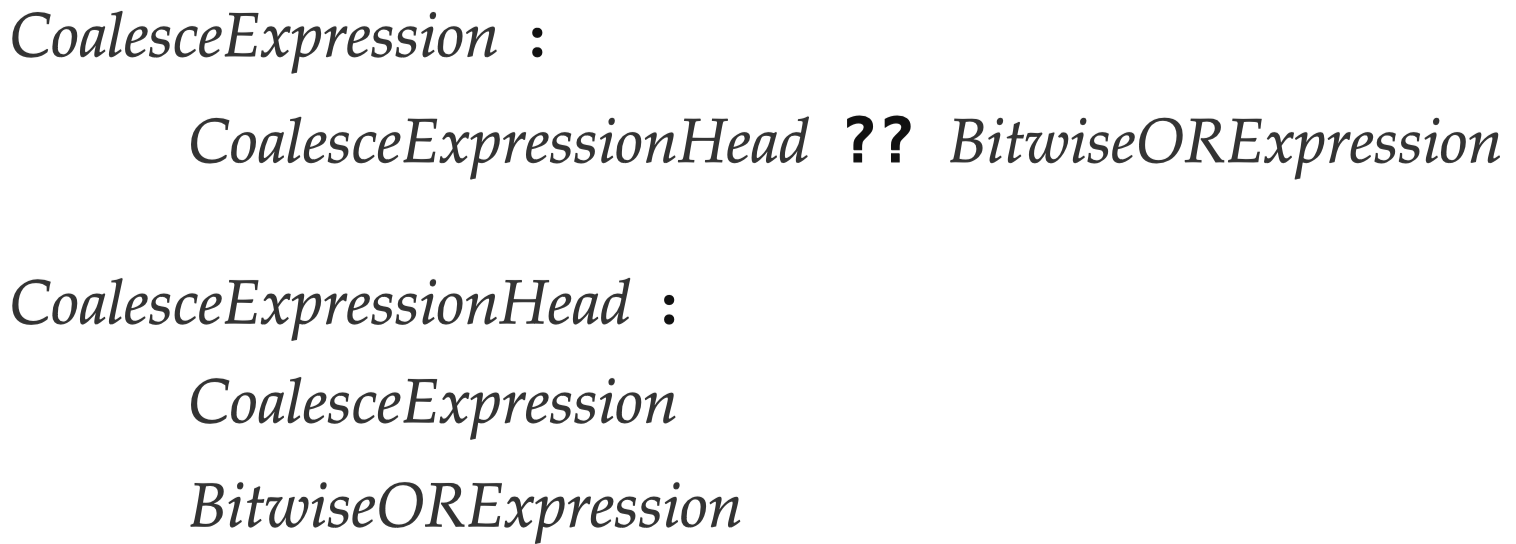
\includegraphics[width=.8\columnwidth]{img/coalesce-prod.png}
  \caption{A JavaScript syntactic production for coalesce expressions}
  \label{fig:coalesce-prod}
\end{figure}




\subsubsection{Concrete Semantics}

The concrete semantics $\sem{\prog}$ of an $\ires$ program $\prog = (\istset,
\getinst, \getnext)$ is defined as follows:
\[
  \sem{\prog} = \{ \st \in \stset \mid \ist \in \istset \wedge \ist \trans^* \st \}
\]
where $\trans^*$ denotes one or more repetition of $\trans$, and $\st \trans
\st'$ if and only if $\st = (\lab, \_, \_, \_)$ and $\sem{\getinst(\lab)}(\st) =
\st'$. Another way to represent the concrete semantics is to define a transfer
function $\transfer: \powerset{\stset} \rightarrow \powerset{\stset}$:
\[
  \sem{\prog} = \lim_{n \rightarrow \infty}\transfer^n(\istset)
\]
where $\transfer(S) = \{ \st' \mid \st \in S \wedge \st \trans \st' \}$.  Now,
we define the denotational semantics of expressions, instructions, and
functions.

\paragraph{Expressions} We define the denotational semantics of expressions with
the following form:
\[
  \framebox{$\sem{\expr}: \stset \rightarrow \valset$}
\]
For each expression $\expr \in \exprset$, its semantics $\sem{\expr}$ takes a
state and returns a value as the result of expression. We define four different
cases in the semantics of expressions as
follows:
\begin{itemize}
  \item \underline{Primitive Values}:
    \[
      \sem{\pval}(\st) = \pval
    \]

  \item \underline{Operations}:
    \[
      \sem{\op \kwrl \expr_1, \cdots, \expr_n \kwrr}(\st) =
      \op(\val_1, \cdots, \val_n)
    \]
    where $\forall 1 \leq j \leq n. \; \sem{\expr_k}(\st) = \val_j$

  \item \underline{Variable Lookups}:
    \[
      \sem{\varx}(\st) = \env(\varx)
    \]
    where $\st = (\_, \_, \_, \env)$

  \item \underline{Field Lookups}:
    \[
      \sem{\expr_0 \kwsl \expr_1 \kwsr}(\st) = \val
    \]
    where
    \[
      \begin{array}{l@{~}c@{~}ll}
        \val_0 &=& \sem{\expr_0}(\st) &\wedge\\
        \val_1 &=& \sem{\expr_1}(\st) &\wedge\\
        \st &=& (\_, \_, \heap, \_) &\wedge\\
        \val &=& \left\{
          \begin{array}{ll}
            \heap(\addr)(\str)
            & \text{if} \; \val_0 = \addr \wedge \val_1 = \str\\

            \tree_j
            & \text{if} \; \val_0 = \ty_k \langle \tree_1, \cdots, \tree_n
            \rangle \wedge \val_1 = j\\
          \end{array}
        \right.\\
      \end{array}
    \]
\end{itemize}

\paragraph{Instructions} We define the denotational semantics of instructions
with the following form:
\[
  \framebox{$\sem{\inst}: \stset \rightarrow \stset$}
\]
For each instruction $\inst \in \instset$, its semantics $\sem{\inst}$ takes a
state and returns an updated state. We define six different cases in the
semantics of instructions as follows:

\begin{itemize}
  \item \underline{Variable Assignments}:
    \[
      \sem{\varx \kweq \expr}(\st) =
      (\getnext(\lab), \ctxts, \heap, \env[\varx \mapsto \val])
    \]
    where $\sem{\expr}(\st) = ((\lab, \ctxts, \heap, \env), \val)$

  \item \underline{Field Assignments}:
    \[
      \sem{\expr_0 \kwsl \expr_1 \kwsr \kweq \expr_2}(\st) =
      (\getnext(\lab), \ctxts, \heap[\addr \mapsto \obj'], \env)
    \]
    where
    \[
      \begin{array}{l@{~}c@{~}ll}
        \sem{\expr_0}(\st) &=& (\st', \addr) &\wedge\\
        \sem{\expr_1}(\st') &=& (\st'', \str) &\wedge\\
        \sem{\expr_2}(\st'') &=& ((\lab, \ctxts, \heap, \env), \val) &\wedge\\
        \obj &=& \heap(\addr) &\wedge\\
        \obj' &=& \obj[\str \mapsto \val]\\
      \end{array}
    \]

  \item \underline{Object Allocations}:
    \[
      \sem{\varx \kweq \kwcl \kwcr}(\st) =
      (\lab, \ctxts, \heap[\addr \mapsto \varnothing], \env[\varx \mapsto
      \addr])
    \]
    where $\st = (\lab, \ctxts, \heap, \env) \wedge \addr \not\in
    \text{Domain}(\heap)$

  \item \underline{Function Calls}:
    \[
      \sem{\varx \kweq \expr \kwrl \expr_1 \cdots \expr_n \kwrr}(\st) =
      (\lab_\varf, \ctxt :: \ctxts, \heap, \env')
    \]
    where
    \[
      \begin{array}{l@{~}c@{~}ll}
        \sem{\expr}(\st) &=& (\st_0, \kwdef \; \kwrl \varx_1, \cdots, \varx_n
        \kwrr \; \lab_\varf) &\wedge\\
        \sem{\expr_j}(\st_{j-1}) &=& (\st_j, \val_j) \;
        [\forall 1 \leq j \leq n] &\wedge\\
        \st_n &=& (\lab, \ctxts, \heap, \env) &\wedge\\
        \env' &=& [\varx_1 \mapsto \val_1, \cdots, \varx_n \mapsto \val_n]
        &\wedge\\
        \ctxt &=& (\getnext(\lab), \env, \varx)\\
      \end{array}
    \]

  \item \underline{Branches}:
    \[
      \sem{\kwif \; \expr \; \lab_\vart \; \lab_\varf}(\st) =
      \left\{
        \begin{array}{ll}
          (\lab_\vart, \ctxts, \heap, \env) & \text{if} \; \val = \true\\
          (\lab_\varf, \ctxts, \heap, \env) & \text{if} \; \val = \false\\
        \end{array}
      \right.
    \]
    where $\sem{\expr}(\st) = ((\lab, \ctxts, \heap, \env), \val)$

  \item \underline{Returns}:
    \[
      \sem{\kwret \; \expr}(\st) = (\lab, \ctxts, \heap, \env[\varx \mapsto
      \val])
    \]
    where $\sem{\expr}(\st) = ((\_, (\lab, \env, \varx) :: \ctxts, \heap, \_),
    \val)$
\end{itemize}


\subsection{Syntactic Views}

A syntactic view $\atree \in \atreeset$ is an abstract JavaScript AST with
abstract tree nodes $\anodeset$:
\[
  \begin{array}{l@{~}c@{~}l@{~}c@{~}l}
    \atreeset &\ni& \atree &::=& \ty_k \langle \anode^* \rangle \mid \ty\\
    \anodeset &\ni& \anode &::=& \str \mid \atree\\
  \end{array}
\]
where $\ty$ denotes all ASTs whose nonterminal symbol $\ty$. We define the
concretization of abstract trees $\atreegamma: \atreeset \rightarrow
\powerset{\treeset}$ and that of abstract nodes $\anodegamma: \anodeset
\rightarrow \powerset{\nodeset}$ as follows:
\[
  \begin{array}{lcl}
    \atreegamma(\ty_k \langle \anode_1, \cdots, \anode_n \rangle) &=&
    \{ \ty_k \langle \node_1, \cdots, \node_n \rangle \mid \node_j \in
    \anodegamma(\anode_j) \}\\

    \atreegamma(\ty) &=&
    \{ \tree \in \treeset \mid \tree = \ty_k \langle \cdots \rangle \}\\

    \anodegamma(\str) &=& \{ \str \}\\

    \anodegamma(\atree) &=& \atreegamma(\atree)\\
  \end{array}
\]
% \[
%   \begin{array}{lcl}
%     \anode \order \anode' &\Leftrightarrow& \left\{
%       \begin{array}{ll}
%         \anode = \anode' &\vee\\
% 
%         \anode' = \ty &\vee\\
% 
%         (\anode = \atree \wedge \anode' = \atree' \wedge \atree \order
%         \atree')\\
%       \end{array}
%     \right.\\
% 
%     \atree \order \atree' &\Leftrightarrow& \left\{
%       \begin{array}{ll}
%         \atree = \atree' &\vee\\
% 
%         \atree' = \treetop &\vee\\
% 
%         \begin{array}{@{}l@{}}
%           \atree = \ty_k \langle \atree_1, \cdots, \atree_n \rangle \wedge
%           \atree' = \ty_k \langle \atree'_1, \cdots, \atree'_n \rangle \wedge\\
%           \forall j. \; \tree_j \order \tree'_j\\
%         \end{array}\\
%       \end{array}
%     \right.\\
% 
%     \atree \join \atree' &=& \left\{
%       \begin{array}{ll}
%         \atree' & \text{if} \; \atree \order \atree'\\
% 
%         \atree & \text{if} \; \atree \revorder \atree'\\
% 
%         \ty_k \langle \atree''_1, \cdots, \atree''_n \rangle &
%         \text{if} \; \atree = \ty_k \langle \atree_1, \cdots, \atree_n \rangle
%         \wedge\\&
%         \phantom{\text{if} \;} \atree = \ty_k \langle \atree_1, \cdots, \atree_n
%         \rangle \wedge\\&
%         \phantom{\text{if} \;} \forall j. \; \atree''_j = \atree_j
%         \join \atree'_j\\
%         \treetop & \text{otherwise}\\
%       \end{array}
%     \right.\\
%   \end{array}
% \]
Moreover, we define abstract subtree relation $\asubtree \subseteq \atreeset
\times \treeset$:
\[
  \atree \; \asubtree \; \tree' \iff \exists \tree \in \atreegamma(\atree). \;
  \tree \subtree \tree'
\]
to filter out JavaScript programs not related to a given syntactic view.
Similar to $\getsubs(\tree)$, an abstract helper function $\agetsubs(\atree)$
denotes abstract tree nodes that are syntactic views when $\atree = \ty_k
\langle \cdots \rangle$.



\subsection{Partial Evaluation}

We define a \textit{partial evaluation} $\peval{-}: \progset \rightarrow
\atreeset \rightarrow \progset$ of $\ires$ programs to specialize JavaScript
semantics with a given syntactic view:
\[
  \peval{\prog}(\atree) = \transform{\prog} \circ \asem{\prog} (\atree)
\]
It takes a syntactic view $\atree \in \atreeset$ to restrict arguments of the
corresponding \esalg{Evaluation} function. Then, it performs a static analysis
$\asem{-}$ of a given program $\prog$ with the syntactic view $\atree$ and
transforms the program using $\transform{-}$ with the analysis result
$\asem{\prog}(\atree)$ to produce a specialized $\ires$ program.  Since the
\esalg{Evaluation} of $\ty$ might one or more $\ires$ functions, we only define
the partial evaluation when $\atree = \ty_k \langle \cdots \rangle$.  Now, we
define the static analysis and program transformation of $\ires$ programs and
prove the semantics preservation of the partial evaluation consisting of them.


\subsubsection{Static Analysis}

The static analysis $\asem{\prog}(\atree)$ performs an abstract
interpretation~\cite{ai1977, ai1992} to abstract concrete semantics under the
given given syntactic view $\atree$.  We first define abstract domains of
states, calling contexts, environments, and values as follows:
\begin{itemize}
  \item \underline{Abstract States}:
    $\aelemset = \amctxtset \times \atctxtset \times \afsenvset$
    \[
      \begin{array}{lcl}
        \aelemgamma(\amctxt, \atctxt, \afsenv) &=&
        \amctxtgamma(\amctxt) \cup
        (\atctxtgamma(\atctxt) \cap \afsenvgamma(\afsenv))\\

        (\amctxt, \atctxt, \afsenv) \order
        (\amctxt', \atctxt', \afsenv') &\Leftrightarrow&
        (\amctxt \order \amctxt') \wedge
        (\atctxt \order \atctxt') \wedge
        (\afsenv \order \afsenv')\\

        (\amctxt, \atctxt, \afsenv) \join (\amctxt', \atctxt', \afsenv') &=&
        (\amctxt \join \amctxt', \atctxt \join \atctxt', \afsenv \join \afsenv')\\
      \end{array}
    \]

  \item \underline{Merged Calling Contexts}:
    $\amctxtset = \powerset{\labset}$
    \[
      \begin{array}{lcl}
        \amctxtgamma(\amctxt) &=& \{ \st \in \stset \mid
          \st = (\lab, [\ctxt_1, \cdots, \ctxt_n], \_, \_) \wedge\\&&

          \phantom{\{ \st \in \stset \mid}
          \exists 1 \leq j \leq n. \; \ctxt_j = (\lab_j, \_, \_) \wedge\\&&

          \phantom{\{ \st \in \stset \mid}
          \lab_j \in \amctxt
        \}\\

        \amctxt \order \amctxt' &\Leftrightarrow&
        \amctxt \subseteq \amctxt\\

        \amctxt \join \amctxt' &=&
        \amctxt \cup \amctxt\\
      \end{array}
    \]

  \item \underline{Target Calling Contexts}:
    $\atctxtset = \powerset{\labset \times \funcset}$
    \[
      \begin{array}{lcl}
        \atctxtgamma(\atctxt) &=& \{ \st \in \stset \mid
          \st = (\lab_0, [\ctxt_1, \cdots, \ctxt_n], \_, \_) \wedge\\&&

          \phantom{\{ \st \in \stset \mid}
          \forall 1 \leq j \leq n. \; \ctxt_j = (\lab_j, \_, \_) \wedge\\&&

          \phantom{\{ \st \in \stset \mid}
          \exists 0 \leq m \leq n. \; \getfunc(\lab_m) = \ty_k.\eval \wedge\\&&

          \phantom{\{ \st \in \stset \mid}
          \forall 1 \leq j \leq m. \; (\lab_j, \getfunc{\lab_{j-1}}) \in \atctxt
        \}\\

        \atctxt \order \atctxt' &\Leftrightarrow& \atctxt \subseteq \atctxt\\

        \atctxt \join \atctxt' &=& \atctxt \cup \atctxt'\\
      \end{array}
    \]

  \item \underline{Flow-Sensitive Abstract Environments}:
    $\afsenvset = \labset \rightarrow \aenvset$
    \[
      \begin{array}{lcl}
        \afsenvgamma(\afsenv) &=& \{ \st \in \stset \mid
          \st = (\lab, \_, \_, \_) \wedge \st \in \aenvgamma(\afsenv(\lab))
        \}\\

        \afsenv \order \afsenv' &\Leftrightarrow&
        \forall \lab \in \labset. \; \afsenv(\lab) \order \afsenv'(\lab)\\

        \afsenv \join \afsenv' &=&
        \lambda \lab \in \labset. \; \afsenv(\lab) \join \afsenv'(\lab)\\
      \end{array}
    \]

  \item \underline{Abstract Environments}:
    $\aenvset = \varset \rightarrow \aenvset$
    \[
      \begin{array}{lcl}
        \aenvgamma(\aenv) &=& \{ \st \in \stset \mid
          \forall \varx \in \varset. \;
          \sem{\varx}(\st) \in \avalgamma(\aenv(\varx))
        \}\\

        \aenv \order \aenv' &\Leftrightarrow&
        \forall \varx \in \varset. \;
        \aenv(\varx) \order \aenv'(\varx)\\

        \aenv \join \aenv' &=&
        \lambda \varx \in \varset. \;
        \aenv(\varx) \join \aenv'(\varx)\\
      \end{array}
    \]

  \item \underline{Abstract Values}: $\avalset = \valset \uplus \atreeset \uplus
    \{ \top, \bot,  \}$
    \[
      \begin{array}{lcl}
        \avalgamma(\aval) &=& \left\{
          \begin{array}{ll}
            \{ \val \} & \text{if} \; \aval = \val\\
            \atreegamma(\atree) & \text{if} \; \aval = \atree\\
            \valset & \text{if} \; \aval = \top\\
            \varnothing & \text{if} \; \aval = \bot\\
          \end{array}
        \right.\\

        \aval \order \aval' &\Leftrightarrow& \left\{
          \begin{array}{ll}
            \aval = \bot \vee \aval' = \top \vee \aval = \aval' & \vee\\
            \aval = \atree \wedge \aval' = \atree' \wedge
            \atree \order \atree' &\vee\\
            \aval = \tree \wedge \aval' = \atree' \wedge \tree \in
            \atreegamma(\atree')\\
          \end{array}
        \right.\\

        \aval \join \aval' &=& \left\{
          \begin{array}{ll}
            \aval' & \text{if} \; \aval \order \aval'\\
            \aval & \text{if} \; \aval \revorder \aval'\\
            \top & \text{otherwise}\\
          \end{array}
        \right.\\
      \end{array}
    \]
\end{itemize}

An abstract state $\aelem \in \aelemset$ is a triple of a merged and target call
edges and a flow-sensitive abstract environment.  A merged calling context
$\amctxt \in \amctxtset$ is a set of call labels representing merged function
calls. A target calling context $\atctxt \in \atctxtset$ is a set of possible
static call edges from labels to function, and it represents the scope of static
analysis. To more precisely represent states in target calling contexts, we
define a flow-sensitive abstract environment $\afsenv \in \afsenvset$. It is
a mapping from labels to abstract environments to represents the shape of
environments in each label. An abstract environment $\aenv \in \aenvset$ is a
mapping from variables to abstract values to describe values stored in
variables. An abstract value $\aval \in \avalset$ is a static value $\val$, a
syntactic view $\atree$, a dynamic value $\top$, or nothing $\bot$.  Now, we
define abstract semantics of expressions, instructions, and programs.

\paragraph{Expressions} We first define abstract semantics of expressions as
follows:
\[
  \framebox{$\asem{\expr}: \aenvset \rightarrow \avalset$}
\]
\begin{itemize}
  \item \underline{Primitive Values}:
    \[
      \asem{\pval}(\aenv) = \pval
    \]
  \item \underline{Operations}:
    \[
      \asem{\op \kwrl \expr_1, \cdots, \expr_n \kwrr}(\aenv) = \aval
    \]
    where
    \[
      \begin{array}{l@{~}c@{~}l@{~}l}
        \asem{\expr_j}(\aenv) &=& \aval_j \; [\forall 1 \leq j \leq n]
        &\wedge\\
        \aval &=& \left\{
          \begin{array}{ll}
            \bot & \text{if} \; \exists j. \; \aval_j = \bot\\

            \op(\val_1, \cdots, \val_n) &
            \text{if} \; \forall j. \; \aval_j = \val_j\\

            \top & \text{otherwise}\\
          \end{array}
        \right.\\
      \end{array}
    \]
  \item \underline{Variable Lookups}:
    \[
      \asem{\varx}(\aenv) = \aenv(\varx)
    \]
  \item \underline{Field Lookups}:
    \[
      \asem{\expr_0 \kwsl \expr_1 \kwsr}(\aenv) = \aval
    \]
    where
    \[
      \begin{array}{l@{~}c@{~}l@{~}l}
        \asem{\expr_0}(\aenv) &=& \aval_0 &\wedge\\
        \asem{\expr_1}(\aenv) &=& \aval_1 &\wedge\\
        \aval &=& \left\{
          \begin{array}{ll}
            \tree_j & \text{if} \;
            \aval_0 = \ty_k \langle \tree_1, \cdots, \tree_n \rangle \wedge
            \aval_1 = j\\

            \atree_j & \text{if} \;
            \aval_0 = \ty_k \langle \atree_1, \cdots, \atree_n \rangle \wedge
            \aval_1 = j\\

            \top & \text{otherwise}\\
          \end{array}
        \right.\\
      \end{array}
    \]
\end{itemize}

\paragraph{Instructions} Then, we define the abstract semantics of instructions
as follows:
\[
  \framebox{$\asem{\inst}: \amctxtset \times \atctxtset \times \labset \times
    \aenvset \rightarrow
  \aelemset$}
\]
\begin{itemize}
  \item \underline{Variable Assignments}:
    \[
      \asem{\varx \kweq \expr}(\amctxt, \atctxt, \lab, \aenv) =
      (\amctxt, \atctxt, [\getnext(\lab) \mapsto \aenv[\varx \mapsto \aval]])
    \]
    where $\aval = \asem{\expr}(\aenv)$

  \item \underline{Field Assignments}:
    \[
      \asem{\expr_0 \kwsl \expr_1 \kwsr \kweq \expr_2}(\amctxt, \atctxt, \lab, \aenv) =
      (\amctxt, \atctxt, [\getnext(\lab) \mapsto \aenv])
    \]

  \item \underline{Object Allocations}:
    \[
      \asem{\varx \kweq \kwcl \kwcr}(\amctxt, \atctxt, \lab, \aenv) =
      (\amctxt, \atctxt, [\getnext(\lab) \mapsto \aenv[\varx \mapsto \top]])
    \]

  \item \underline{Function Calls}:
    \[
      \asem{\varx \kweq \expr \kwrl \expr_1 \cdots \expr_n \kwrr}(\amctxt,
      \atctxt, \lab, \aenv) = (\amctxt', \atctxt', \afsenv)
    \]
    where
    \[
      \begin{array}{l@{~}c@{~}ll}
        \aval &=& \asem{\expr}(\aenv) &\wedge\\
        \aval_j &=& \asem{\expr_j}(\aenv) \; [\forall 1 \leq j \leq n] &\wedge\\
        (\amctxt', \atctxt') &=& \left\{
          \begin{array}{ll}
            (\amctxt, \atctxt \cup \{ (\lab, \func) \} &
            \text{if} \; \aval = \func \wedge \exists j. \; \aval_j \neq \top\\

            (\amctxt \cup \{ \lab \}, \atctxt) &
            \text{otherwise}
          \end{array}
        \right.\\
        \afsenv &=& [ \lab_\func \mapsto \aenv_\func \mid
        (\lab, \func) \in \atctxt' \wedge\\&&

        \phantom{[\lab_\func \mapsto \aenv_\func \mid \;}
        \func = \kwdef \; \kwrl \varx_1, \cdots, \varx_n \kwrr
        \; \lab_\func \wedge\\&&

        \phantom{[\lab_\func \mapsto \aenv_\func \mid \;}
        \aenv_\func = [\varx_1 \mapsto \aval_1, \cdots,
        \varx_n \mapsto \aval_n] ]\\
      \end{array}
    \]

  \item \underline{Branches}:
    \[
      \asem{\kwif \; \expr \; \lab_\vart \; \lab_\varf}(\amctxt, \atctxt, \lab, \aenv) =
      (\amctxt, \atctxt, \afsenv')
    \]
    where
    \[
      \begin{array}{lcl}
        \aval &=& \asem{\expr}(\aenv)\\

        \afsenv &=& \left\{
          \begin{array}{ll}
            [\lab_\vart \mapsto \aenv] & \text{if} \; \true \in
            \avalgamma(\aval)\\
            \varnothing & \text{otherwise}\\
          \end{array}
        \right.\\

        \afsenv' &=& \left\{
          \begin{array}{ll}
            \afsenv[\lab_\varf \mapsto \aenv] & \text{if} \; \false \in
            \avalgamma(\aval)\\
            \afsenv & \text{otherwise}\\
          \end{array}
        \right.\\
      \end{array}
    \]

  \item \underline{Returns}:
    \[
      \asem{\kwret \; \expr}(\amctxt, \atctxt, \lab_0, \aenv) =
      (\amctxt, \atctxt, \afsenv)
    \]
    where
    \[
      \begin{array}{lcl}
        \aval &=& \asem{\expr'}(\aenv)\\

        \func &=& \getfunc(\lab_0)\\
        R &=& \{ (\getnext(\lab), \varx) \mid
          (\lab, \func) \in \atctxt \wedge\\

          && \phantom{\{ (\getnext(\lab), \varx) \mid}
          \getinst(\lab) = \varx \kweq \expr^\lab (\expr^\lab_1 \cdots \expr^\lab_n)
        \}\\

        \afsenv &=& \lambda \lab \in \labset. \; \left\{
          \begin{array}{ll}
            [\varx \mapsto \aval]
            & \text{if} \; (\lab, \varx) \in R\\

            \varnothing
            & \text{otherwise}\\
          \end{array}
        \right.\\
      \end{array}
    \]
\end{itemize}

\paragraph{Programs} Finally, we define the abstract semantics of programs with
a given syntactic view.  We define it as the least fixed point of the abstract
transfer function with the target initial abstract state depending on the given
syntactic view:
\[
  \asem{\prog}(\atree) = \lim_{n \rightarrow
  \infty}(\atransfer)^n(\iaelem(\atree))
\]
where
\begin{itemize}
  \item \underline{Abstract Transfer Function}: $\atransfer: \aelemset
    \rightarrow \aelemset$
    \[
      \atransfer(\aelem) = \aelem \join \sem{\amctxt} \wedge
      \bigjoin_{\lab \in \labset}{\asem{\getinst(\lab)}(\amctxt, \atctxt, \lab,
      \afsenv(\lab))}
    \]
    where $\aelem = (\amctxt, \atctxt, \afsenv)$ and $\sem{\amctxt} = (\amctxt,
    \atctxt, [\lab \mapsto \aenv_\lab \mid \lab \in \amctxt \wedge
    \getinst(\lab) = \varx = \expr(\cdots) \wedge \aenv_\lab = [\varx \mapsto
    \top]])$.
  \item \underline{Target Initial Abstract State}: $\iaelem:
    \atreeset \rightarrow \aelemset$
    \[
      \iaelem(\atree) = (\varnothing, \varnothing, \afsenv)
    \]
    where \[
      \begin{array}{lcl}
        \atree &=& \ty_k \langle \cdots \rangle\\

        \agetsubs(\atree) &=& [\atree_1, \cdots, \atree_n]\\

        \ty_k.\eval &=& \lambda \kwdef \; \kwrl \varx_1, \cdots, \varx_n \kwrr
        \; \lab\\

        \aenv &=& [\varx_1 \mapsto \atree_1, \cdots, \varx_n \mapsto
        \atree_n]\\

        \afsenv &=& [\lab \mapsto \aenv]\\
      \end{array}
    \]
\end{itemize}


\subsubsection{Transformations}

Using the analysis result, we define transformations for expressions,
instructions, and programs.

\paragraph{Expressions} We first define the transformation of expressions as
follows:

\[
  \framebox{$\transform{\expr}: \aenvset \rightarrow \exprset$}
\]
\[
  \transform{\expr}(\aenv) = \left\{
    \begin{array}{ll}
      \pval & \text{if} \; \asem{\expr}(\aenv) = \pval\\
      \expr & \text{otherwise}\\
    \end{array}
  \right.
\]

\paragraph{Instructions} Then, we define the transformation of instructions
as follows:
\[
  \framebox{$\transform{\inst}: \aenvset \rightarrow \instset$}
\]
\begin{itemize}
  \item \underline{Variable Assignments}:
    \[
      \transform{\varx \kweq \expr}(\aenv) =
      \varx \kweq \expr'
    \]
    where $\expr' = \transform{\expr}(\aenv)$

  \item \underline{Field Assignments}:
    \[
      \transform{\expr_0 \kwsl \expr_1 \kwsr \kweq \expr_2}(\aenv) =
      \expr'_0 \kwsl \expr'_1 \kwsr \kweq \expr'_2
    \]
    where
    \[
      \begin{array}{l@{~}c@{~}ll}
        \expr'_0 = \transform{\expr_0}(\aenv) &\wedge\\
        \expr'_1 = \transform{\expr_1}(\aenv) &\wedge\\
        \expr'_2 = \transform{\expr_2}(\aenv)\\
      \end{array}
    \]
  \item \underline{Object Allocations}:
    \[
      \transform{\varx \kweq \kwcl \kwcr}(\aenv) =
      \varx \kweq \kwcl \kwcr
    \]

  \item \underline{Function Calls}:
    \[
      \transform{\varx \kweq \expr \kwrl \expr_1 \cdots \expr_n \kwrr}(\aenv) =
      \varx \kweq \expr' \kwrl \expr'_1 \cdots \expr'_n \kwrr
    \]
    where
    \[
      \begin{array}{l@{~}c@{~}ll}
        \expr' = \transform{\expr}(\aenv) &\wedge\\
        \expr'_k = \transform{\expr_k}(\aenv) \; [\forall 1 \leq k \leq
        n]\\
      \end{array}
    \]

  \item \underline{Branches}:
    \[
      \transform{\kwif \; \expr \; \lab_\vart \; \lab_\varf}(\aenv) =
      \kwif \; \expr' \; \lab_\vart \; \lab_\varf
    \]
    where $\expr' = \transform{\expr}(\aenv)$

  \item \underline{Returns}:
    \[
      \transform{\kwret \; \expr}(\aenv) =
      \kwret \; \expr'
    \]
    where $\expr' = \transform{\expr}(\aenv)$
\end{itemize}

\paragraph{Programs} Finally, we define the program transformation as follows:
\[
  \framebox{$\transform{\prog}: \aelemset \rightarrow \progset$}
\]
\[
  \transform{\prog}(\amctxt, \atctxt, \afsenv) = (\istset, \getfunc, \getinst',
  \getnext)
\]
where $\prog = (\istset, \getfunc, \getinst, \getnext)$ and $\getinst' =
\getinst[\lab \mapsto \inst_\lab \mid \aenv = \afsenv(\lab) \neq \epsilon \wedge
\inst_\lab = \transform{\getinst(\lab)}(\aenv)]$.



\subsubsection{Cleanup Algorithm}

\todo

\begin{itemize}
  \item perform a syntactic def-use analysis
  \item remove unnecessary variable assignments
  \item remove unreachable instructions
\end{itemize}


\subsubsection{Semantics Preservation}

% We first define a helper function $\entrystset: \atreeset \rightarrow
% \powerset{\stset}$ to define the set of entry states for a given syntactic view
% $\atree = \ty_k \langle \cdots \rangle$:
% \[
%   \begin{array}{l@{~}l}
%     \entrystset(\atree) = \{ \st \in \stset \mid &
%       \st = (\lab, \_, \_, \env) \wedge\\&
% 
%       \env = [\varx_0 \mapsto \atree, \varx_1 \mapsto \atree_1, \cdots, \varx_n
%       \mapsto \atree_n]
%     \}\\
%   \end{array}
% \]
% where $\ty_k.\eval = \kwdef \; \kwrl \varx_0, \cdots, \varx_n \kwrr \lab$ and
% $\agetsubs(\atree) = [\atree_1, \cdots, \atree_n]$. Then, we define a restricted
% semantics $\rsem{-}: \progset \rightarrow \atreeset \rightarrow
% \powerset{\stset}$ as follows:
% \[
%   \begin{array}{l@{~}l@{~}l}
%     \rsem{\prog}(\atree) = \{ \st \in \stset \mid&
%       \st' \in \sem{\prog} \cap \entrystset(\atree) &\wedge\\&
%       \st' \trans^* \st  &\wedge\\&
%       \st' = (\_, \ctxts', \_, \_) &\wedge\\&
%       \st = (\_, \ctxts, \_, \_) &\wedge\\&
%       \ctxts \postfix \ctxts
%     \}
%   \end{array}
% \]
% where $x \postfix y$ denotes that a sequence $y$ is a postfix of a sequence $x$.

\todo

\begin{theorem}[Soundness of $\asem{-}$]
  For a given program $\prog \in \progset$ and a syntactic view $\atree \in
  \atreeset$. Assume that $\asem{\prog}(\atree) = \aelem = (\amctxt, \atctxt,
  \afsenv)$. Then, the following condition should be satisfied:
  \[
    \rsem{\prog}(\atree, \atctxt) \subseteq \gamma(\aelem)
  \]
\end{theorem}
\begin{proof}
  \todo
\end{proof}

\begin{lemma}[Soundness of $\atransfer$]
  The abstract transfer function $\atransfer$ is a sound approximation of the
  transfer function $\transfer$ by satisfying the following condition:
  \[
    \forall \aelem \in \aelemset. \;
    \transfer \circ \gamma(\aelem) \subseteq \gamma \circ \atransfer(\aelem)
  \]
\end{lemma}
\begin{proof}
  \todo
\end{proof}

\begin{theorem}[Semantics Preservation of $\transform{-}$]
  \[
    \todo
  \]
\end{theorem}
\begin{proof}
  \todo
\end{proof}

\todo
